\documentclass{exam}
\usepackage{graphicx}
\usepackage{amsmath}
\newcommand\mycolv[1]{\begin{bmatrix}#1\end{bmatrix}}

\begin{document}

\pagestyle{headandfoot}
\runningheadrule
\firstpageheader{Robot Control}{First Exam}{February 6, 2023}
\runningheader{Robot Control}{First Exam \thepage/\numpages}{February 6, 2023}
\firstpagefooter{}{}{}
\runningfooter{}{}{}

\begin{itemize}
    \item The theory part of the exam will be held from 9:00 AM to 10:00 AM and is worth 20 points.
    \item The practical part will be held from 10:20 AM to 1:30 PM and is worth 30 points.
    \item For the theoretical part of the exam, you are allowed to refer to your personal written notes. (no iPads)
    \item During the practical part of the exam, you are permitted to use your own equipment and consult online documentation. However, using sites such as Stack Overflow is not allowed.
    \item There are four tasks in theory part to be completed. Each task must be solved on a separate piece of paper and signed by you to confirm its completion.
\end{itemize}

Theory problems:

\begin{questions}
%\qformat{Question \thequestion: \thequestiontitle\dotfill\thepoints}
\question


We have two identical pinhole cameras with focal lengths
$5$ and optical centers $x = 300$, $y = 200$.
Cameras have no distortions.

\begin{parts}
\part[1]
  What is the camera matrix?
\part[2]
  Let's assume two cameras' optic axes are parallel and the second
  camera is shifted by \texttt{x=0,y=1,z=0} with respect to the first
  camera. What is the pixel disparity (distance in pixels) between the
  points on images that correspond to a point in the 3D space with
  coordinates \texttt{(5,\ 5,\ 5)} in the first camera's coordinate frame.
\end{parts}

\vspace*{1cm}
\hrule
\vspace*{0.5cm}

\titledquestion{Linearization around Fixed Points}

Recall from the classes that we can model population growth using the so
called logistic model:

\[\dot{x} = x(P_{max}-x)\]

where $x$ is the population size and $P_{max}$ is the population
limit above which the environment becomes resource scarse.

Now consider the more complicated situation when two species are
competing with each other. In this situation the change in population
depends also on the amount of interactions between two populations:

\[\dot{x} = x(P_{max}-x) - a \cdot g(x,y)\]

where $y$ is the current population size of the second species, $a$ is
some parameter and $g$ is some function of $x$ and $y$ describing the interactions between species.

Your task is to use the above model for a competition between rabbits and
wolves - population sizes denoted by $r$ and $w$ respectively. You have
to:

\begin{parts}
\part[1] write the ODEs describing the system assuming that:

  \begin{itemize}
  \item
    the number of interactions between two populations is simply the
    number of (rabbit, wolf) pairs that can be created in the environment
  \item
    $P_{max}$ is equal to $4$ for rabbits and $3$ for wolves
  \item
    $a$ is equal to 2 for rabbits and 1 for wolves
  \item
    your state is $\vec{x} = [r, w]^T$
  \end{itemize}
\part[1] find fixed points of the created system
\part[3] linearize dynamics of the system around those fixed points
\end{parts}

\vspace*{1cm}
\hrule
\vspace*{0.5cm}

\question
Given the visual description of the kinematic chain (figure \ref{fig}), consisting of:

\begin{enumerate}
\def\labelenumi{\arabic{enumi}.}
\item
  prismatic joint attached to base with actuation \(d_1\) from 0 to 1
  right
\item
  link: \(a_1\) right, \(a_2\) up, \(a_3\) right
\item
  revolute joint with actuation \(\theta\) from 0 to \(2\pi\)
\item
  link: \(a_4\) up, \(a_5\) right
\item
  prismatic joint with actuation \(d_2\) from 0 to 1 downwards
\item
  link: \(a_6\) down, ending with the end-effector
\end{enumerate}

\begin{figure}[!ht]
\centering
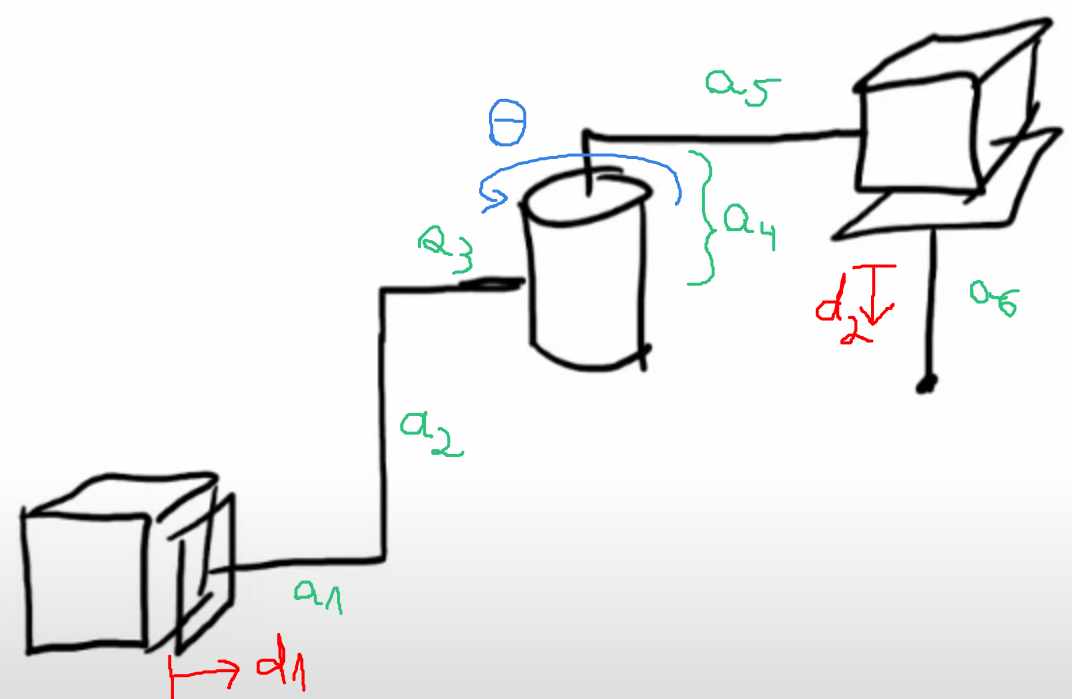
\includegraphics[scale=0.2]{theory-2/theory-2.png}
\caption{Kinematic chain for problem 2}
\label{fig}
\end{figure}

do the following:

\begin{parts}
\part[1]
  Find the forward kinematics \(FK(d_1, \theta, d_2)\) of the robot
\part[1]
  Find the workspace of the robot with fixed \(d_1 = 0\)
\part[1]
  Find the inverse kinematics $$IK$$ of the robot with fixed \(d_1 = 0\), i.e.
  whenever \(FK(0, \theta, d_2) = (x, y, z)\) we have \(IK(x, y, z) = (\theta, d_2)\)
\part[1]
  Assign frames to the joints of the kinematic chain using the
  DH-convention
\part[2]
  Create the DH-table for the kinematic chain including the actuation of
  joints
\end{parts}

\vspace*{1cm}
\hrule
\vspace*{0.5cm}


\newpage

\titledquestion{Transformations}

In this task we have a robot that is equipped with a 3D camera,
and the camera's frame is represented by the coordinate system $C$.
The global coordinate system is represented by the coordinate system $W$.
The position and orientation of the camera (transformation from $W$ to $C$)
is given by a homogeneous transformation matrix $H^W_C$.

\begin{parts}
\part[2]
Suppose that a point $P$ has coordinates $P^C$ in the camera frame $C$.
Write the expression for the point $P^W$, that is the same point $P$ expressed in the world frame.
Use homogeneous coordinates.

\part[2]

In this step you cannot use the matrix inverse operator $M^{-1}$ directly.
Use your knowledge about the inverse of the homogeneous transformation matrix.

The point $P$ is the same one as in the previous step. Now there is also a point $Q$.
The difference between the two points is given by the vector $\delta^W$
in the global frame $W$, meaning $P^W + \delta^W = Q^W$ (all in the global frame $W$).
Write an expression for the coordinates of the second point $Q$ in the camera frame $C$, that is $Q^C$.

Express the result using $P^C$, $\delta^W$ and component blocks of $H^W_C$.

\part[2]

Use the result from two previous points to find the coordinates of point $Q$ in the camera frame,
assuming the following values:

$$
H^W_C = \begin{bmatrix} \cos(45^\circ) & -\sin(45^\circ) & 0 & 1 \cr
\sin(45^\circ) & \cos(45^\circ) & 0 & 2 \cr
0 & 0 & 1 & 3 \cr
0 & 0 & 0 & 1 \end{bmatrix}
$$


$$
P^C = \mycolv{ p^C_x \cr p^C_y \cr p^C_z} = \mycolv{3 \cr 2 \cr 1}
$$


$$
\delta^W = \mycolv{d_x \cr d_y \cr d_z} = \mycolv{2 \cr 0 \cr -1}
$$
\end{parts}
\end{questions}
    
\end{document}
